\documentclass[twoside, 11pt]{article}

\usepackage{amsmath}
\usepackage{amssymb}
\usepackage[colorlinks=true, citecolor=blue, linkcolor=black]{hyperref}
\usepackage{listings}
\usepackage{xcolor}
\usepackage{graphicx}

\usepackage{calrsfs}

%\usepackage[sc]{mathpazo} % Use the Palatino font
\usepackage[T1]{fontenc} % Use 8-bit encoding that has 256 glyphs
\linespread{1} % Line spacing - Palatino needs more space between lines
\usepackage{microtype} % Slightly tweak font spacing for aesthetics

\usepackage[hmarginratio=1:1,top=32mm,columnsep=20pt]{geometry} % Document margins
\usepackage{multicol} % Used for the two-column layout of the document
\renewcommand{\figurename}{\bfseries\scshape Fig.}
\renewcommand{\tablename}{\bfseries\scshape Table}
\usepackage[hang, small,labelfont=sc,up,textfont=normalfont,up]{caption} % Custom captions under/above floats in tables or figures
\usepackage{float} % Required for tables and figures in the multi-column environment - they need to be placed in specific locations with the [H] (e.g. \begin{table}[H])
\usepackage{hyperref} % For hyperlinks in the PDF

\usepackage{listings}
\lstset{language=C++,
				backgroundcolor=\color{black!5},
                basicstyle=\scriptsize ,
                keywordstyle=\color{blue}\ttfamily,
                stringstyle=\color{red}\ttfamily,
                commentstyle=\color{green}\ttfamily,
                morecomment=[l][\color{magenta}]{\#},
                tabsize = 1,
}

\usepackage{abstract} % Allows abstract customization
\renewcommand{\abstractnamefont}{\normalfont\bfseries} % Set the "Abstract" text to bold
\renewcommand{\abstracttextfont}{\normalfont\small\itshape} % Set the abstract itself to small italic text

\usepackage{titlesec} % Allows customization of titles
%\renewcommand\thesection{\textbf{\Roman{section}}} % Roman numerals for the sections
%\renewcommand\thesubsection{\roman{subsection}} % Roman numerals for subsections
\titleformat{\section}[block]{\bf\Large\scshape\centering}{\thesection.}{1em}{} % Change the look of the section titles
\titleformat{\subsection}[block]{\bf\large\scshape\centering}{\thesubsection}{1em}{} % Change the look of the section titles
\titleformat{\subsubsection}[block]{\bf\normalsize\scshape\centering}{\thesubsubsection}{1em}{}

\usepackage{fancyhdr} % Headers and footers
\pagestyle{fancy} % All pages have headers and footers
\fancyhead{} % Blank out the default header
\fancyfoot{} % Blank out the default footer
\fancyhead[CO]{FYS3150 - Computational physics $~ \cdot ~$ Project 4} % Custom header text
\fancyhead[CE]{Ole Gunnar Johansen $~ \cdot ~$ Candidate number 16}
\fancyfoot[C]{\small\thepage} % Custom footer text

%----------------------------------------------------------------------------------------
%	TITLE SECTION
%----------------------------------------------------------------------------------------

\title{\vspace{-15mm}\fontsize{16pt}{13pt}\selectfont\textbf{Solving the 2D Ising model using the Metropolis algorithm}} % Article title

\author{
\large
Ole Gunnar Johansen\\[0mm]%\thanks{A thank you or further information}\\[2mm] % Your name
Candidate number 16 \\
\normalsize University of Oslo \\[0mm] % Your institution
\normalsize \href{mailto:olegjo@ulrik.uio.no}{olegjo@student.matnat.uio.no} % Your email address
\vspace{5mm}
}
\date{}

\renewcommand{\d}{\mathrm{d}}

\newcommand{\HUSK}[1]{{\color{red}\Large\bfseries ~[#1]}}
\usepackage{caption}
\usepackage{subcaption}
\begin{document}
\maketitle % Insert title
\thispagestyle{fancy} % All pages have headers and footers


\begin{abstract}

\noindent
In this project, I have employed the Metropolis algorithm to solve the two dimensional Ising model. First, I look at a small system and solve this analytically before I implement the algorithm and solve it numerically. I then use this to approximate the critical temperature of phase transition of the lattice.

I also make a note on an interesting result which may be the manifestation on the ferromagnetic Weiss domains we can observe in nature. 

\end{abstract}

%\begin{multicols}{1}

\section{Introduction}
	In statistical physics, the Ising model provides us with a good model of the ferromagnetic phenomenon. It deals with a collection of spins arranged in a lattice where each spin is quantized up or down and is allowed to interact with its nearest neighbours. 

	While the one dimensional Ising model is quite easy to solve analytically, the two dimensional Ising model is more difficult. It was first solved analytically by Norwegian-American physicist Lars Onsager mid-20th century in what is called the Onsager limit. The numerical solution is, however, much simpler and gives us a good insight in how the system approaches equilibrium
	
	In this project, I have solved the two dimensional Ising model with no external magnetic field and periodic boundary conditions using the Metropolis algorithm to find the heat capacity, magnetic susceptibility as well as various expectation values for the system.
	

	
	All source code can be found at my github\footnote{\url{https://github.com/olegjo/FYS3150-project-4}}.

\section{Theory/Methods}
	In its simplest form, the total energy of the Ising model can be expressed as
	\begin{align}
		E = -J \sum_{<kl>}^N s_ks_l - \mathcal{B}\sum_k^N s_k
	\end{align}
	where $s = \pm 1$, $N$ is the total number of spins, $J$ is a coupling constant determining the strength of the interaction between neighbouring spins and $\mathcal{B}$ is an external magnetic field. The sum over $<kl>$ indicates that the sum is taken over nearest neighbours only. 
	
	In this project we will address the Ising model without external magnetic field, $\mathcal{B}=0$, and periodic boundary conditions, $s_{N+1}=s_1$. The coupling constant $J=1$. 
	
	\subsection{Analytical solution to a small system}
		The full Ising model for a general $N\times N$ lattice, can be very difficult to solve analytically, but we can solve the $2\times 2$ system quite easily. Assume we have a $2\times 2$ lattice we could make the following visualization of the lattice with periodic boundary conditions
		\begin{table}[H]
			\centering
			\begin{tabular}{c c c c}
				& ${\color{red}\uparrow}$ 	& ${\color{cyan}\uparrow}$ \\\cline{2-3}
				\multicolumn{1}{c|}{${\color{blue}\downarrow}$}	&	${\color{green}\uparrow}$ & \multicolumn{1}{c|}{${\color{blue}\downarrow}$} & ${\color{green}\uparrow}$ \\
				\multicolumn{1}{c|}{${\color{cyan}\uparrow}$}	& ${\color{red}\uparrow}$	&	\multicolumn{1}{c|}{${\color{cyan}\uparrow}$}	&	${\color{red}\uparrow}$		\\\cline{2-3}
				&	${\color{green}\uparrow}$	&	${\color{blue}\downarrow}$		
			\end{tabular}
		\end{table}
		where equal colors means that it is the same spin and the actual lattice is inside the square. 
		
		The partition function for the system is given by
		\begin{align*}
			Z = \sum_{i} e^{-\beta E_i}
		\end{align*}
		where $\beta = 1/kT$, $k$ is the Boltzmann constant and the sum is taken over all stated $i$. The possible energy states of the lattice can be organized as in table~\ref{table: 2 by 2 lattice energy states}. 
		\begin{table}
			\centering
			\caption{Possible energy states of the simple $2\times 2$ Ising model.}
			\label{table: 2 by 2 lattice energy states}
			\begin{tabular}{c|c|c|c}
				No. of spins up		&	Degeneracy	&	Energy/$J$	&	Magnetization	\\ \hline
				4	&	1	&	-8	&	4	\\
				3	&	4	&	0	&	2	\\
				2	&	4	&	0	&	0	\\
				2	&	2	&	8	&	0	\\
				1	&	4	&	0	&	-2	\\
				0	&	1	&	-8	&	-4
			\end{tabular}
		\end{table}
		
		The partition function is then
		\begin{align*}
			Z 	&= e^{8J\beta} + 12e^{0} + e^{8J\beta} + 2e^{-8J\beta} \\
				&= 2\left(e^{8J\beta} + e^{-8J\beta} + 6 \right) \\
				&= \cosh(8J\beta) + 12
		\end{align*}
		
		The expectation value for any discrete variable $A$ is  given by
		\begin{align*}
			\langle A \rangle = \sum_i A_ip_i
		\end{align*}
		where $p_i$ is the probability of $A_i$. In this case, the probability for the energy $E_i$ is
		\begin{align*}
			p_i = \frac{e^{-\beta E_i}}{Z}
		\end{align*}
		Therefore, the expectation value for the energy is 
		\begin{align}
			\langle E \rangle 	&= \frac{1}{Z}\sum_{i=1}^{16} E_i e^{-\beta E_i} \nonumber \\
										&= \frac{1}{Z}\left(-8Je^{8J\beta} + 8Je^{-8J\beta} + 8Je^{-8J\beta} - 8Je^{8J\beta} \right) \nonumber \\
										&= \frac{-8J\sinh(8J\beta)}{\cosh(8J\beta) + 12} \label{eq: L=2 theory <E>} 
		\end{align}
		and the expectation value for the square of the energy is given similarly by
		\begin{align*}
			\langle E^2 \rangle = \frac{64J^2\cosh(8J\beta)}{\cosh(8J\beta) + 12}
		\end{align*}
		The specific heat capacity of the small Ising model is 
		\begin{align}
			C_V = \frac{\sigma_E^2}{kT^2} &= \frac{1}{kT^2}\left(\langle E^2 \rangle - \langle E \rangle^2\right) \label{eq: L=2 theory C_V}
		\end{align}
	
	
		A very similar approach can be done for the magnetization of the system giving
		\begin{align*}
			\langle \mathcal{M} \rangle &= 0 \\
			\langle |\mathcal{M}| \rangle &= \frac{8e^{8J\beta} + 4}{\cosh(8J\beta) + 12} \\
			\langle \mathcal{M}^2 \rangle &= \frac{32e^{8J\beta} + 8}{\cosh(8J\beta) + 12}
		\end{align*}
		leaving us with the following expression for the magnetic susceptibility
		\begin{align}
			\chi = \frac{\sigma_M^2}{kT} = \frac{1}{kT}\left(\langle \mathcal{M}^2 \rangle - \langle |\mathcal{M}| \rangle ^2 \right) \label{eq: L=2 theory chi}
		\end{align}
	\subsection{The Onsager Limit}
		The critical temperature $T_C$ of the system is the temperature below which the system becomes spontaneously magnetized, and above which is doesn't. At $T_C$ we then get a phase shift. It has been shown that the mean magnetization of the system as $T \rightarrow T_C$ scales as\footnote{J. Cardy, Scaling and Renormalization in Statistical Physics (Cambridge University Press, 1996)}
		\begin{align*}
			\langle \mathcal{M} (T) \rangle \sim (T - T_C )^\beta
		\end{align*}
		where $\beta = 1/8$ is called the critical exponent. Similarly for the heat capacity and magnetic susceptibility:
		\begin{align*}
			C_V &\sim |T_C - T|^\alpha \\
			\mathrm{and} \qquad \chi &\sim |T_C - T|^\gamma
		\end{align*}
		where $\alpha = 0$ and $\gamma = 7/4$ are the corresponding critical exponents.
		
		As mentioned, the system experiences no net magnetization at $T > T_C$. That is $\langle \mathcal{M} \rangle = 0$ in this limit. However, any spin can only interact with it nearest neighbours only, but in some way, the system as a whole will tend to a specific state. This gives rise to another important quantity called the correlation length, and it describes how far from a specific spin $i$ one have to go before there will not be any correlation between the spin at the current position and the spin at position $i$. In other words the length within which there is a reasonable probability that a change in spin $i$ will cause a change in any other spin within the correlation length.
		
		For smaller temperatures, a change in one spin will have a small probability of changing any of its nearest spins, and hence the correlation length is small, possibly on the order of the lattice spacing. As the temperature increases, however, the correlation length increases and as it approaches $T_C$. This behaviour can be expressed as another power law
		\begin{align*}
			\xi \sim |T_C - T|^{-\nu}
		\end{align*}
		
		For any finite lattice, the correlation length will be of the order of the lattice size $L$, $\xi = a'L$ where $a'$ is a constant. Assume we approaching the critical temperature $T_C$ with increasingly larger $T<T_C$ for 1) a finite lattice and 2) an infinite lattice. Since the correlation length is proportional to the size of the lattice we have
		\begin{align*}
			\xi \sim (T_C(L) - T)^{-\nu} = a'L \Rightarrow T_C(L) - T = aL^{-1/\nu}
		\end{align*}
		and similarly for the infinite lattice:
		\begin{align*}
			T_C(L=\infty) - T = aL^{-1/\nu} 
		\end{align*}
		Using the exact result $\nu = 1$ we get
		\begin{align*}
			T_C(L) &= aL^{-1} + T
			\mathrm{and} \qquad T_C(L=\infty) = T
		\end{align*}
		which leads to the so-called finite size scaling relation
		\begin{align}
			T_C(L) - T_C(L = \infty) &= aL^{-1/\nu} = aL^{-1} \label{eq: finite size scaling}
		\end{align}
%		 one can then relate the critical temperature, mean magnetization, heat capacity and magnetic susceptibility with the lattice size as follows (respectively):
%		\begin{align*}
%			 \\
%			\langle M(T) \rangle \sim (T - T_C)^\beta &\propto  L^{-\beta/\nu} \\
%			C_V(T) \sim |T_C  - T|^{-\alpha}  &\propto L^{\alpha/\nu} \\
%			\chi(T) \sim |T_C  - T|^{-\gamma} & \propto L^{\gamma/\nu}
%		\end{align*}
%		
		Onsager showed that the exact result is $kT_C/J = 2/\ln(1+\sqrt{2}) \approx 2.269$ with $\nu=1$. This limit is hereby referred to as the Onsager limit.

	
	\subsection{The metropolis algorithm}
		The metropolis algorithm employs the fact that nature always tends towards the lowest energy level. The main gist of the algorithm deployed on the Ising model is to choose a random position in the lattice, try flipping the spin at this position, and if the energy decreases it is assumed that this lowers the total energy of the system and hence takes it closer to an equilibrium state. 
		
		The metropolis is then t be considered as a type of Monte Carlo simulation.
		
		The above outline is, however, somewhat simplified. Since we have a Boltzmann distribution in the probability of the energy states, one should also expect the system to approach equilibrium if some random number $w\in[0,1]$ is lower than $e^{-\beta\Delta E}$ ($<1$), where $\Delta E$ is the change in energy between the current state and the trial state. 
		
		For the two dimensional Ising model, we are constrained to five different values for $\Delta E$, ranging from $\Delta E = -4J$ to $\Delta E = 4J$ with spacing of $2J$. Assume we position ourself at a position in the lattice with a spin up. The trial state is then where this is flipped, so it points down.
		\begin{align*}
			\begin{matrix}
								& \uparrow 						& 					\\ 
				\uparrow 	& {\color{red}\uparrow} & \uparrow 	\\ 
								& \uparrow 						&
			\end{matrix} 
			\qquad \Rightarrow \qquad
			\begin{matrix}
								& \uparrow 						& 					\\ 
				\uparrow 	& {\color{red}\downarrow} & \uparrow 	\\ 
								& \uparrow 						&
			\end{matrix} 
		\end{align*}
		with $\Delta E = 8$. If we then iterate through all possibilities, letting first one of the surrounding spins point down, then two, three and finally four, we find the above mentioned allowed $\Delta E$. 
		
		Using this fact, the code can be sped up dramatically by pre-calculating the different values for $e{-\beta \Delta E}$. If we store these in an array \texttt{w} of length 17, we can then make the call to the random number generator \texttt{ran1} as follows:
		\begin{lstlisting}
if (ran1(&idum) <= w[deltaE + 8]) {
	// accept
}
		\end{lstlisting}
			
		The function \texttt{initialize} initializes the lattice. This can be done in different ways, however the two methods I have used in this project is 1) with all spins initially pointing up, and 2) with a random starting position for the spins.
		
		Ref previous discussion on spontaneous magnetization, one should expect that the system was closer to an equilibrium state if the spins were initially set to be uniformly aligned throughout the lattice for temperature below $T_C$. Since the configuration with spin up is lower energetically, such systems will be initialized by uniform spin up. When looking at systems above $T_C$, however, a random starting configuration may be beneficial. 
		
			
			
\section{Results}
	\subsection{Code verification on the $\mathbf{2\times 2}$ lattice}
		For the $2\times 2$ case, the analytical solution is given by equations \eqref{eq: L=2 theory <E>}, \eqref{eq: L=2 theory C_V} and \eqref{eq: L=2 theory chi}. To verify the program, I compared the analytical solutions with the numerical ones for $T=1$ in units of $kT/J$. Table~\ref{table: L=2 compare theory + numerical} shows such comparison.
		
		It is immediately evident that the numerical and analytical result match for $\langle E \rangle$, however they do not for any of the other quantities. I blame the difference on a computing error, however I have not been able to spot the fault. 
		
		All quantities are given per spin.
		\begin{table}
			\centering
			\caption{Comparison of numerical and analytical solution for a small Ising model. All quantities are per spin.}
			\label{table: L=2 compare theory + numerical}
			\begin{tabular}{c | c | c | c | c}
\# MC Cycles 	&	$\langle E \rangle$	&	$C_V$	&	$\langle |M| \rangle$ 	&	$\chi$ \\ \hline
Analytical 	&	-1.98403			&	0.12678	&	3.96872	&	11.93586 \\
100 		&	-1.90000		&	0.76000		&	0.96500	&	0.10510	\\
1000 		&	-1.99000		&	0.07960		&	0.99650	&	0.01095	\\
10000 		&	-1.99320		&	0.05422		&	0.99770	&	0.00698	\\
100000 		&	-1.99632		&	0.02939		&	0.99881	&	0.00345	\\
1000000 		&	-1.99577		&	0.03377		&	0.99861	&	0.00414	
			\end{tabular}
		\end{table}
	
	\subsection{Stability of the system}
		I switch now to a larger lattice size in order to get a more representing model of reality.
		
		A good way of determining the stability of the system over time is to decide at which point various expectation values are sufficiently stable. The Onsager limit for critical temperature is $T_C \approx 2.269$. The time dependence corresponds here to the total number of Monte Carlo cycles.
		
		Fig.~\ref{fig: expectation values as functions of MCcycles} shows such a plot for one temperature above and below $T_C$ and a clear pattern occurs. If we choose a uniform starting position, there are little or no fluctuations in the expectation values for $T=1<T_C$, which is the expected result because the system is now starting with all its spins pointing up which is the most likely situation at this temperature. When changing to a random starting position, however, the situation is somewhat different. The system is now in a very \textit{unlikely} state and it needs some time to reach the state with the highest probability. 
		
		A similar discussion applies for $T=2.4>T_C$. Now, the uniform starting position is closer to the most likely position and the expectation values settle faster for the random starting position. 
		
		The settling is, however fairly quick no matter which temperature or starting position and it looks like they have settled after around 5000 Monte Carlo cycles.
		
		
		\begin{figure}
			\centering
			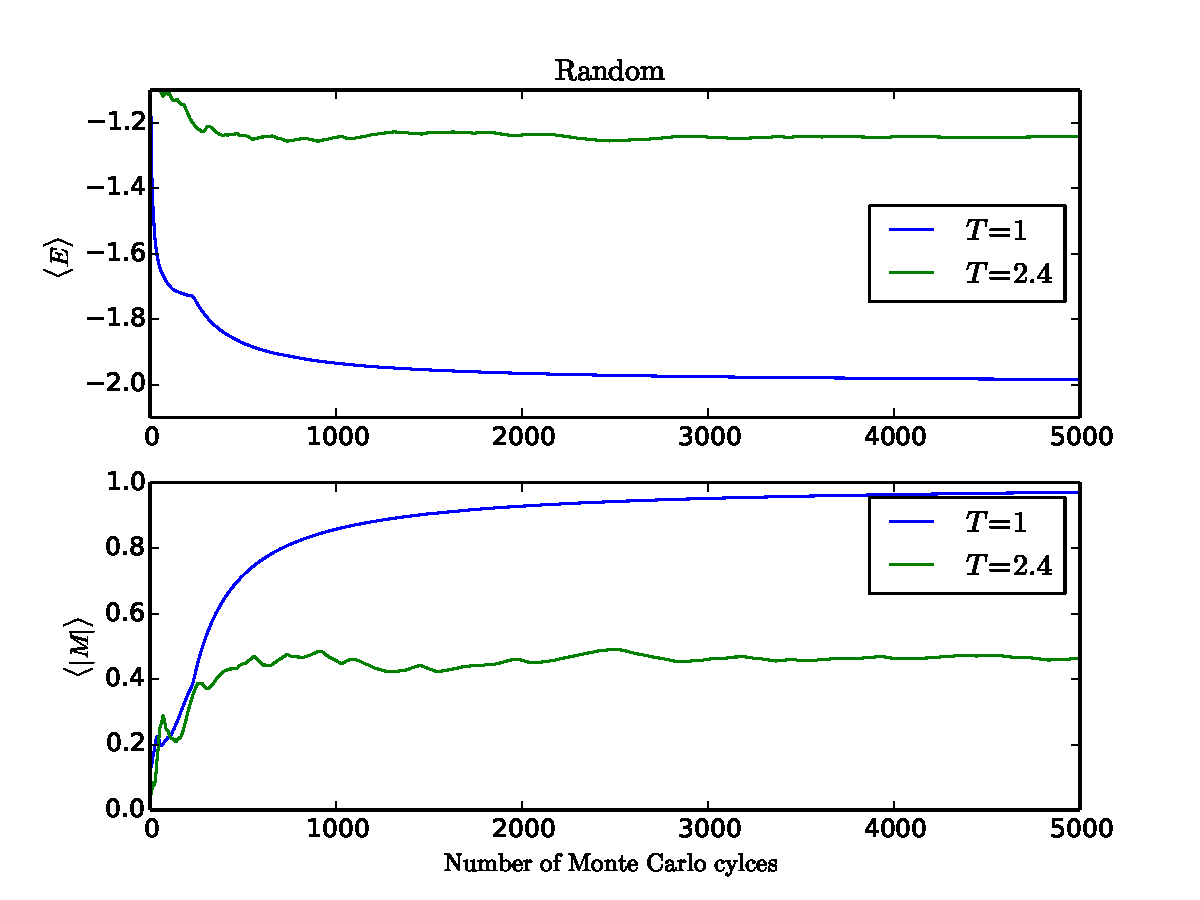
\includegraphics[scale=0.7]{../Results/task_c/task_c_averages_random.pdf}
			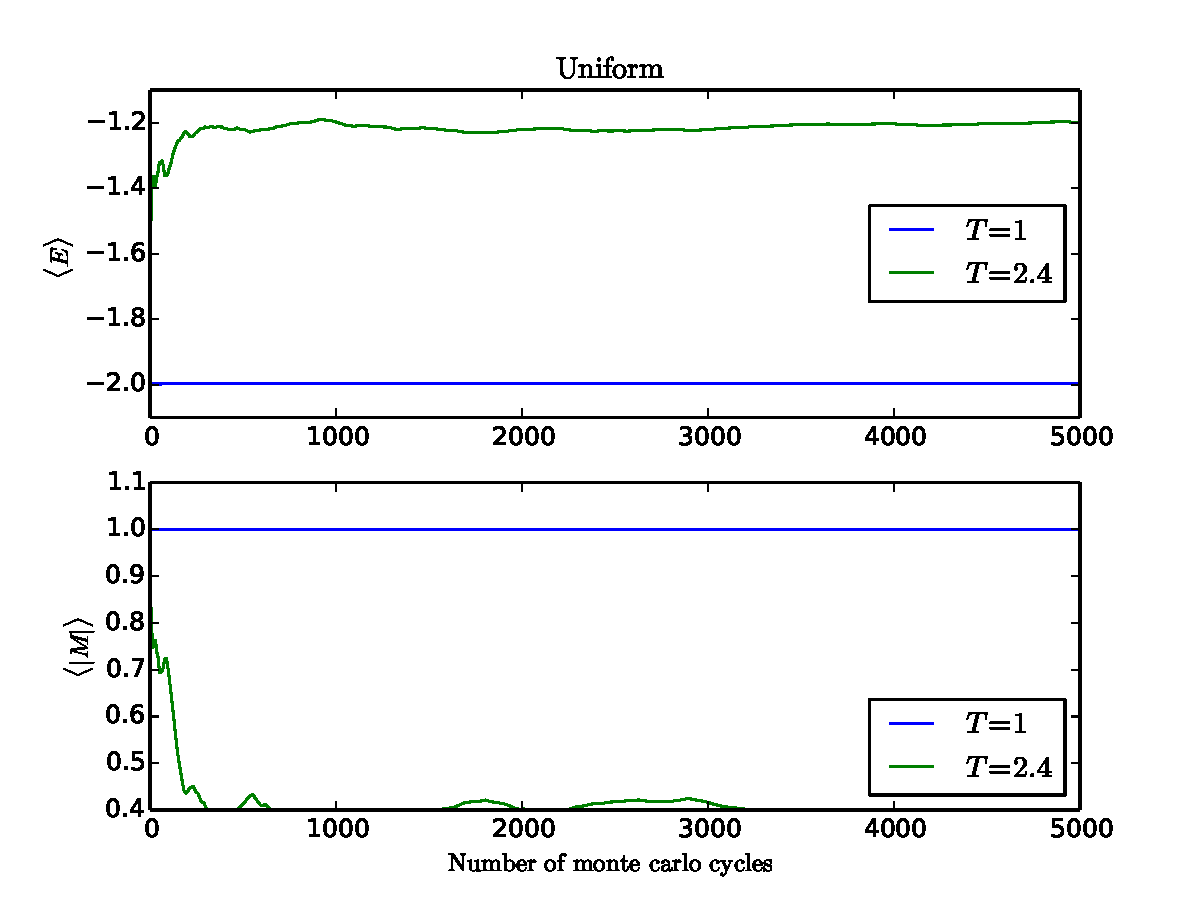
\includegraphics[scale=0.7]{../Results/task_c/task_c_averages_uniform.pdf}
			\caption{$\langle E \rangle$ and $\langle |M| \rangle$ plotted as functions of number of Monte Carlo cycles for $T=1<T_C$ and $T=2.4>T_C$. The top two plots are for a random starting configuration and the bottom two are uniform.}
			\label{fig: expectation values as functions of MCcycles}
		\end{figure}
		
		A quite similar behaviour can be observed if we look at the total number of accepted configurations per Monte Carlo cycle as a function of the number of Monte Carlo cycles. Fig.~\ref{fig: accepted as function of MCcycles} shows this for $T=1$, and, as expected the results stabilize very quickly for the uniform starting position. 
		
		\begin{figure}
			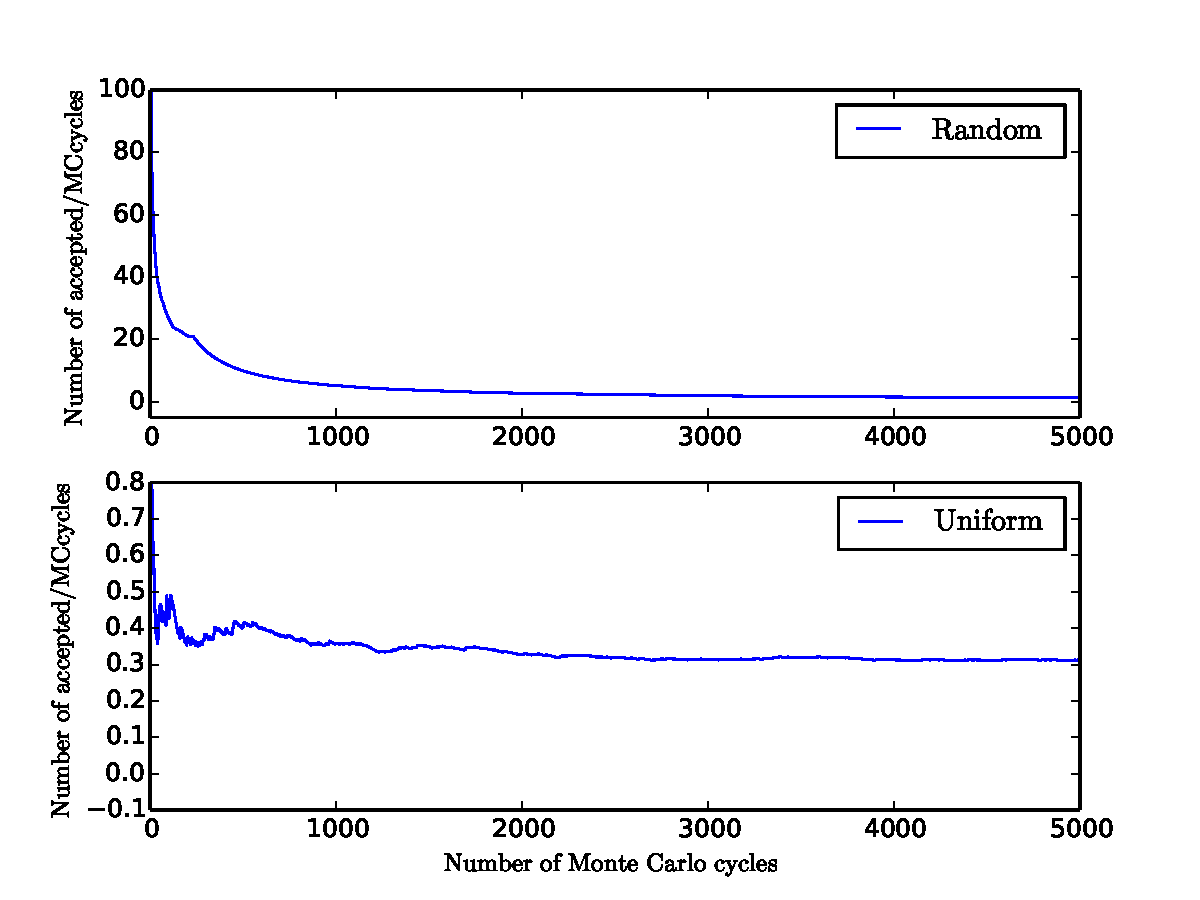
\includegraphics[scale=0.7]{../Results/task_c/task_c_accepted_T1.pdf}
			\caption{Number of accepted Monte Carlo cycles as a function of total number of Monte Carlo cycles for a random and uniform starting position.}
			\label{fig: accepted as function of MCcycles}
		\end{figure}
		
		
	\subsection{The energy of the system}
		Fig.~\ref{fig: P(E) histogram} shows a histogram of the probability distribution of total energy of the system. The energies are sampled after the steady state situation was reached and the corresponding variances are
		\begin{align*}
			\sigma_E(T=1) = 1.952 \qquad \mathrm{and} \qquad \sigma_E(T=2.4) = 160.4
		\end{align*}
		
		\begin{figure}
			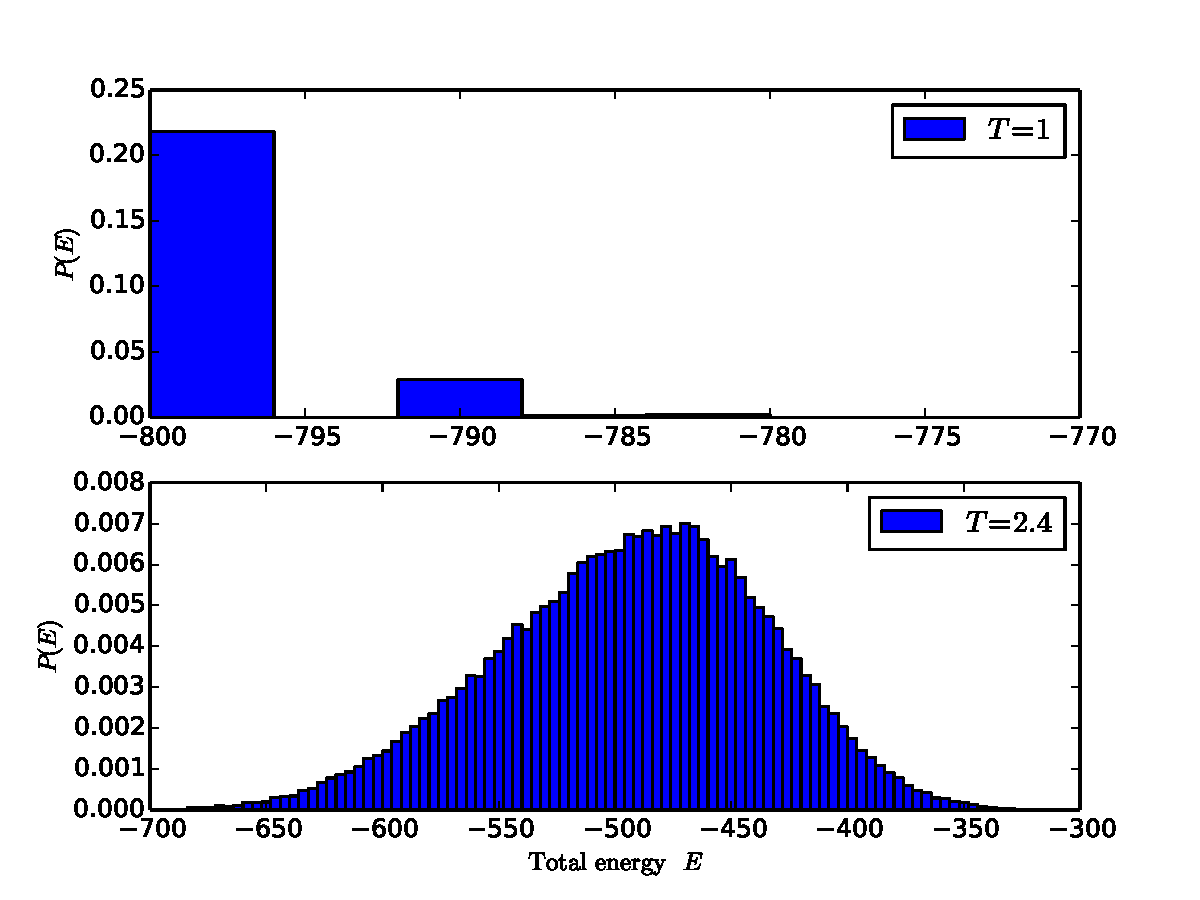
\includegraphics[scale=0.7]{../Results/task_d/task_d_histogram_Uniform.pdf}
			\caption{The total energy $E$ of the system plotted as a probability distribution. }
			\label{fig: P(E) histogram}
		\end{figure}
	
			We see that the system will cluster around a certain value for the specific temperature, and for $T=1$ this is, not surprisingly, at the lowest possible energy. 
			
		\subsection{Phase transitions and infinite lattice size}
			So long I have only looked at finite lattice sizes, and indeed infinite sizes are not possible to simulate. However, I will make an approximation to the infinite lattice by gradually increasing the size of the lattice. Figure~\ref{fig: different lattice sizes} shows a comparison of the different interesting quantities for lattice sized 20, 40, 60, 80 and 100. I have also marked the critical temperature in the Onsager limit with a black vertical line.
			
			The critical temperature of the system is, as we know, where the heat capacity and magnetic susceptibility diverges. We see that as the lattice size increases, the computed critical temperature approaches the true critical temperature in the Onsager limit $kT_C/J = 2.269$.
			
			Table~\ref{table: computed T_C} shows the critical temperatures for the heat capacity and magnetic susceptibility. I used this data to compute the constant of proportionality in eq.~\eqref{eq: finite size scaling} by letting
			\begin{align*}
				T_C(L_1) - aL_1^{-1} = T_C(L_2) - aL_2^{-1}
			\end{align*}
			then comparing all combinations of $L_1$ and $L_2$ in table~\ref{table: computed T_C}. By taking the average $a$, then inserting back in eq.~\eqref{eq: finite size scaling}, I obtained the following for the critical temperature:
			\begin{align*}
				T_C(C_V) = 2.255 \qquad \mathrm{and} \qquad T_C(\chi) = 2.267
			\end{align*}
			
			I do not conclude with any definite answer for why these produce different results, however, I presume they will converge for even larger lattice sizes. 
			\begin{table}
				\centering
				\caption{Computed critical temperatures for the different lattice sizes.}
				\label{table: computed T_C}
				\begin{tabular}{c | c | c}
					$L$		&	$T_C(C_V)$	&	$T_C(\chi)$	\\ \hline
					20		&	2.3	&	2.37	\\
					40		&	2.29	&	2.32	\\
					60		&	2.29	&	2.31	\\
					80		&	2.28	&	2.29	\\
					100		&	2.27	&	2.29	
				\end{tabular}
			\end{table}
			
			\begin{figure}
				\centering
				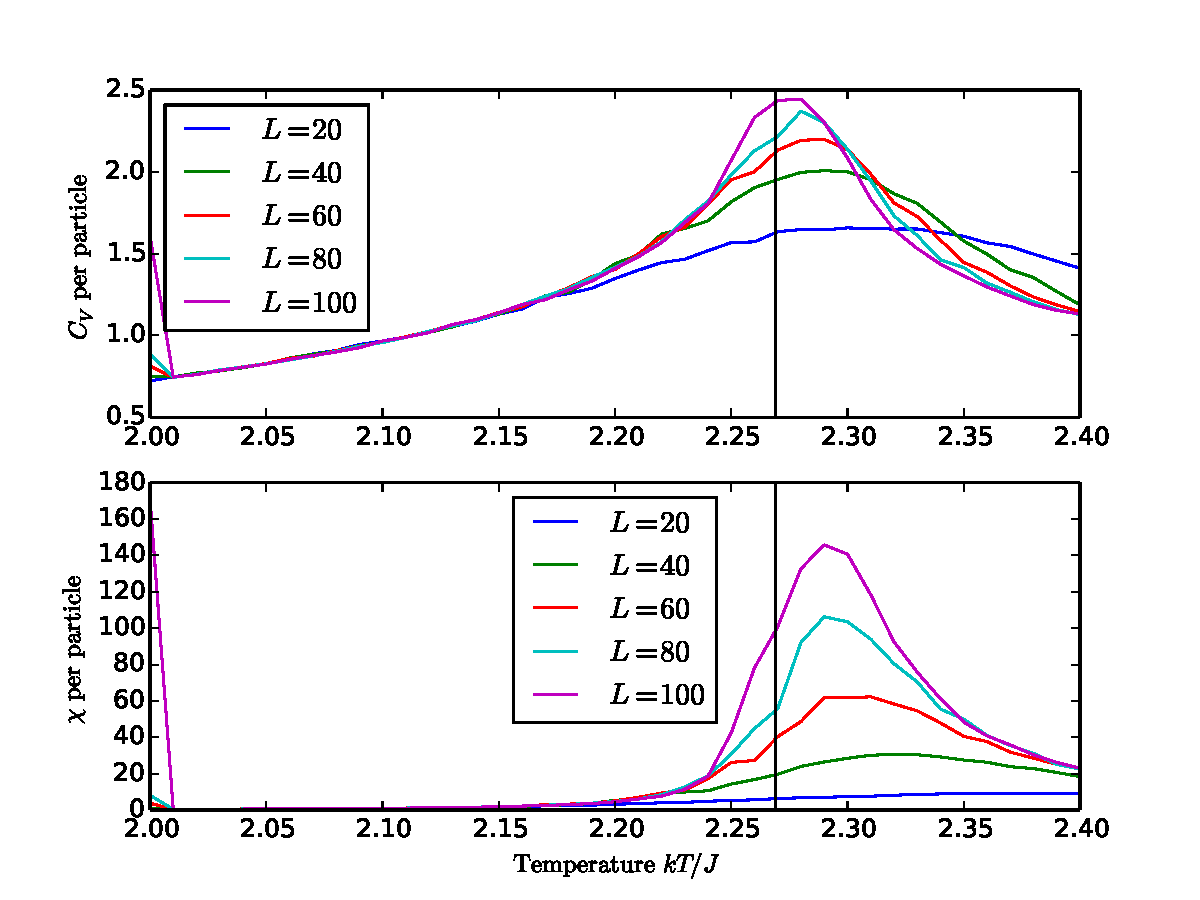
\includegraphics[scale=0.7, clip=true, trim=0 12 0 0]{../Results/task_e/task_e_chi_VS_time_1000000.pdf}
				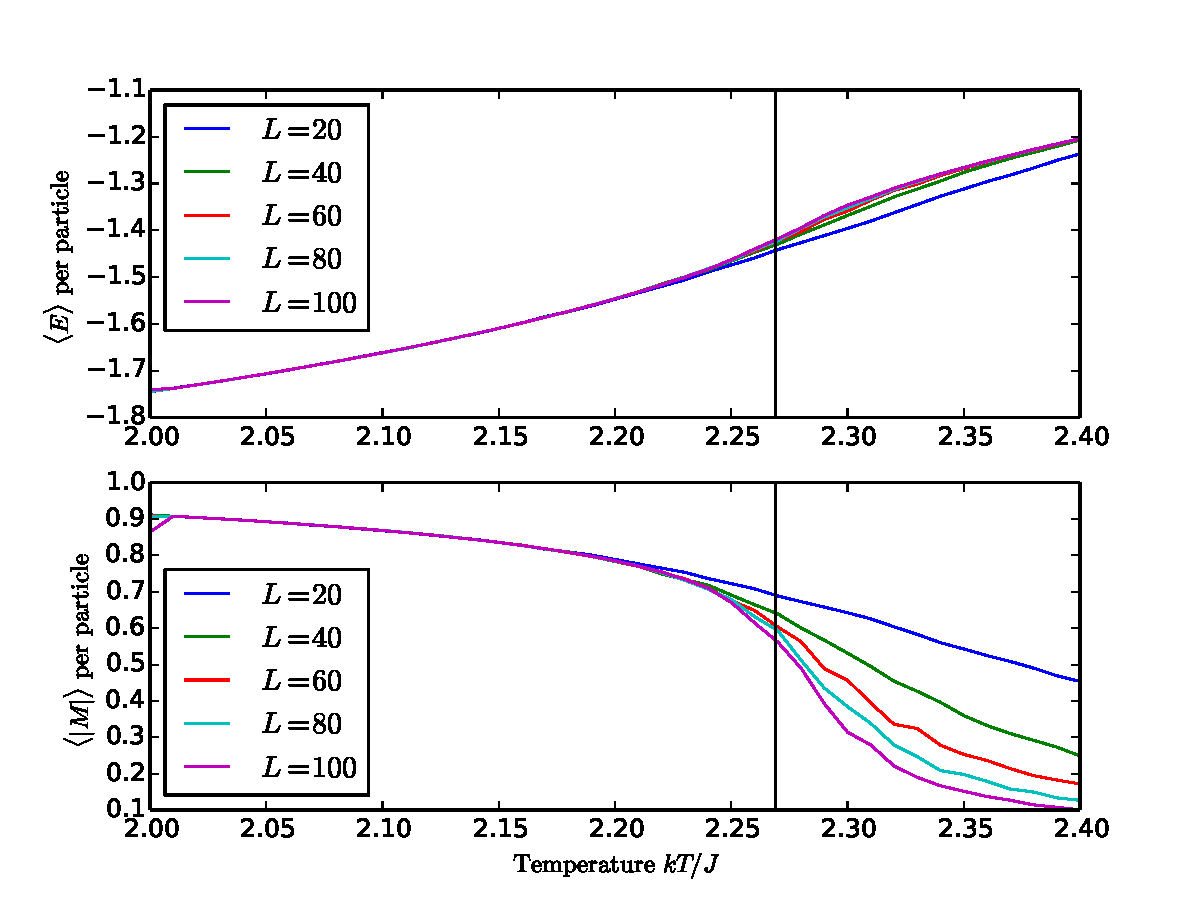
\includegraphics[scale=0.7, clip=true, trim=0 0 0 25]{../Results/task_e/task_e_absMaverage_VS_time_1000000.pdf}
				\caption{Plot of $C_V$, $\chi$, $\langle E \rangle$ and $\langle |M| \rangle$ as functions of temperature for different lattice sizes. The theoretical critical temperature is marked by a black vertical line.}
				\label{fig: different lattice sizes}
			\end{figure}
		
		\subsection{Figure~\ref{fig: expectation values as functions of MCcycles} revisited}
			If we carefully analyse the plot of accepted configurations per MC cycle as a function of MC cycles for the random starting position, fig.~\ref{fig: expectation values as functions of MCcycles}, something quite curious happen. We notice a sudden drop  with an uncontentious first derivative at a point $\sim$200 MC cycles. It looks like the system "feels" it's reached the minimum energy and so does not accept a great number of new configurations until a certain point at which it overcomes some sort of barrier and will again seek towards the true minimum of the system. 
			
			This is a result highly dependent on the starting seed to the random number generator and only some seeds will give the result in question. I therefore changed the seed so that the phenomenon in question would be more prominent. 
			
			To investigate this further, I made an animation\footnote{run \texttt{Results/extra/extra.py} to see the animation.} of the evolution the lattice. Fig.~\ref{fig: animation snapshots} shows three snapshots of this animation. As we can see, the starting position is more or less random (here taken 3 MC cycles into the simulation), but as time goes, the lattice seems to be divided into two sections (cycle=500), since we are dealing with periodic boundary conditions. At this point, the metropolis algorithm will most likely choose a point in the lattice in the middle of either the blue or red area, and any flip of a spin here will result in a higher energy. Only if a spin on the edge between red and blue is chosen, the spin flip will result in a lowering of the energy and thereby acceptance of the new configuration. At cycles=600, this partition is almost gone and the expectation value for energy starts to fall around this point.
			
			 I do not conclude with a definite answer on whether this is only a curiosity with the Ising model or whether real physical systems would also behave this way, however, it is common for ferromagnetic materials to align themselves in domains within the material, where the spins in each domain is aligned. We may therefore be witnessing what is known as Weiss domains. The model does not, however explain why these seem to be stable in reality, but this may be more evident in larger lattices.
			 
			\begin{figure}
			    \centering
			    \begin{subfigure}[b]{0.3\textwidth}
			        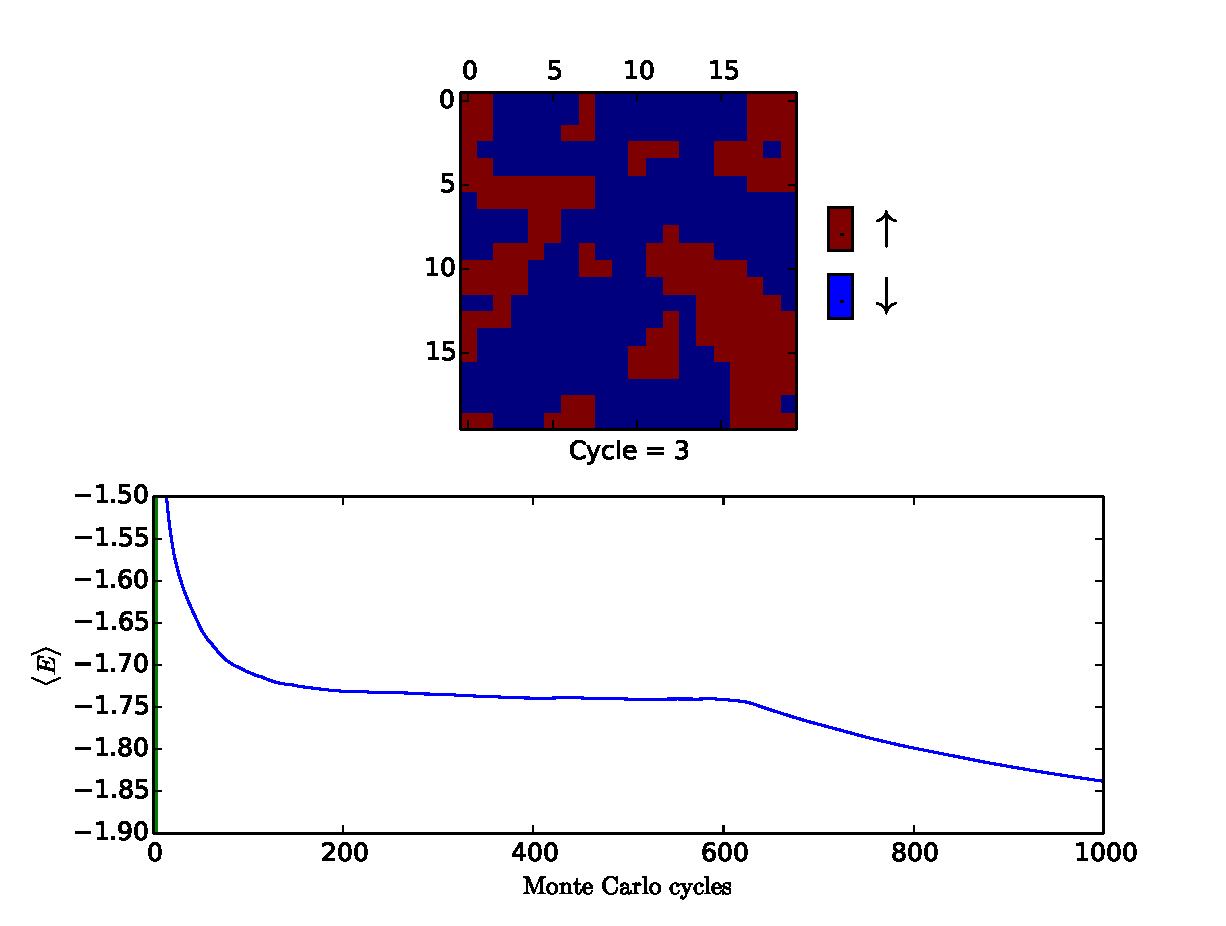
\includegraphics[scale = 0.6, clip=true, trim=210 220 155 0]{../Results/extra/extra_3.pdf}
			    \end{subfigure}
			    ~ 
			    \begin{subfigure}[b]{0.3\textwidth}
			        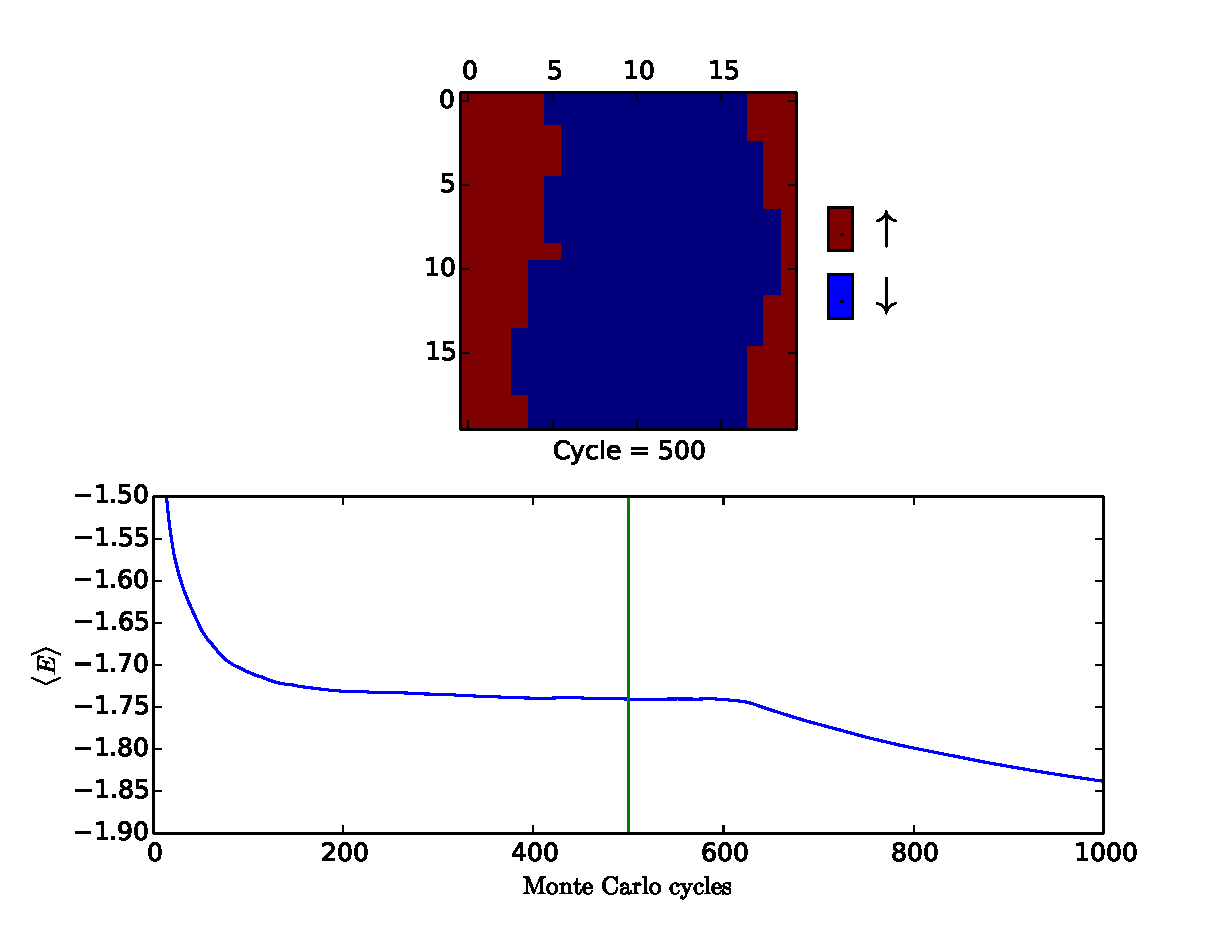
\includegraphics[scale = 0.6, clip=true, trim=210 220 155 0]{../Results/extra/extra_500.pdf}
			    \end{subfigure}
			    ~ 
			    \begin{subfigure}[b]{0.3\textwidth}
			        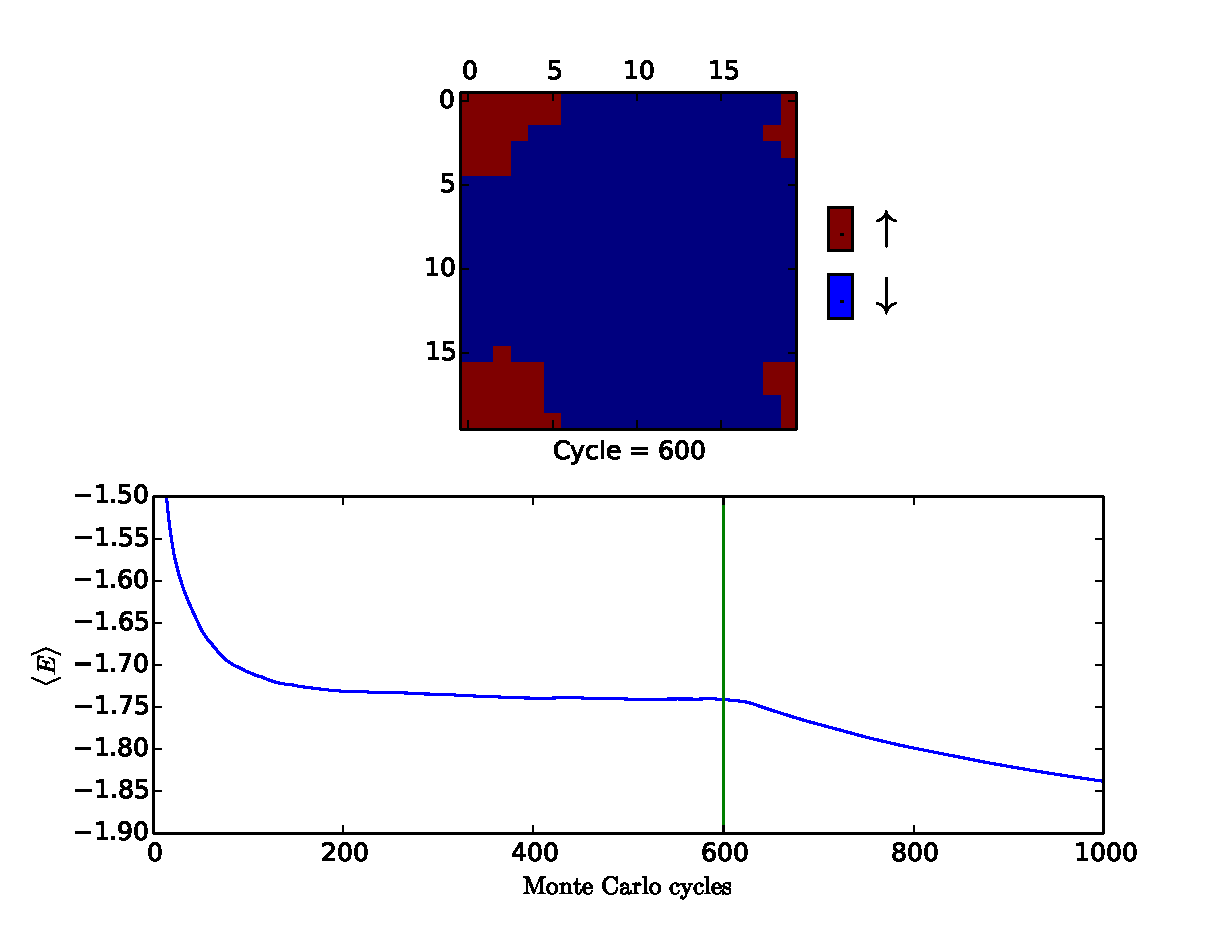
\includegraphics[scale = 0.6, clip=true, trim=210 220 155 0]{../Results/extra/extra_600.pdf}
			    \end{subfigure}
			    \begin{subfigure}[b]{\textwidth}
			    	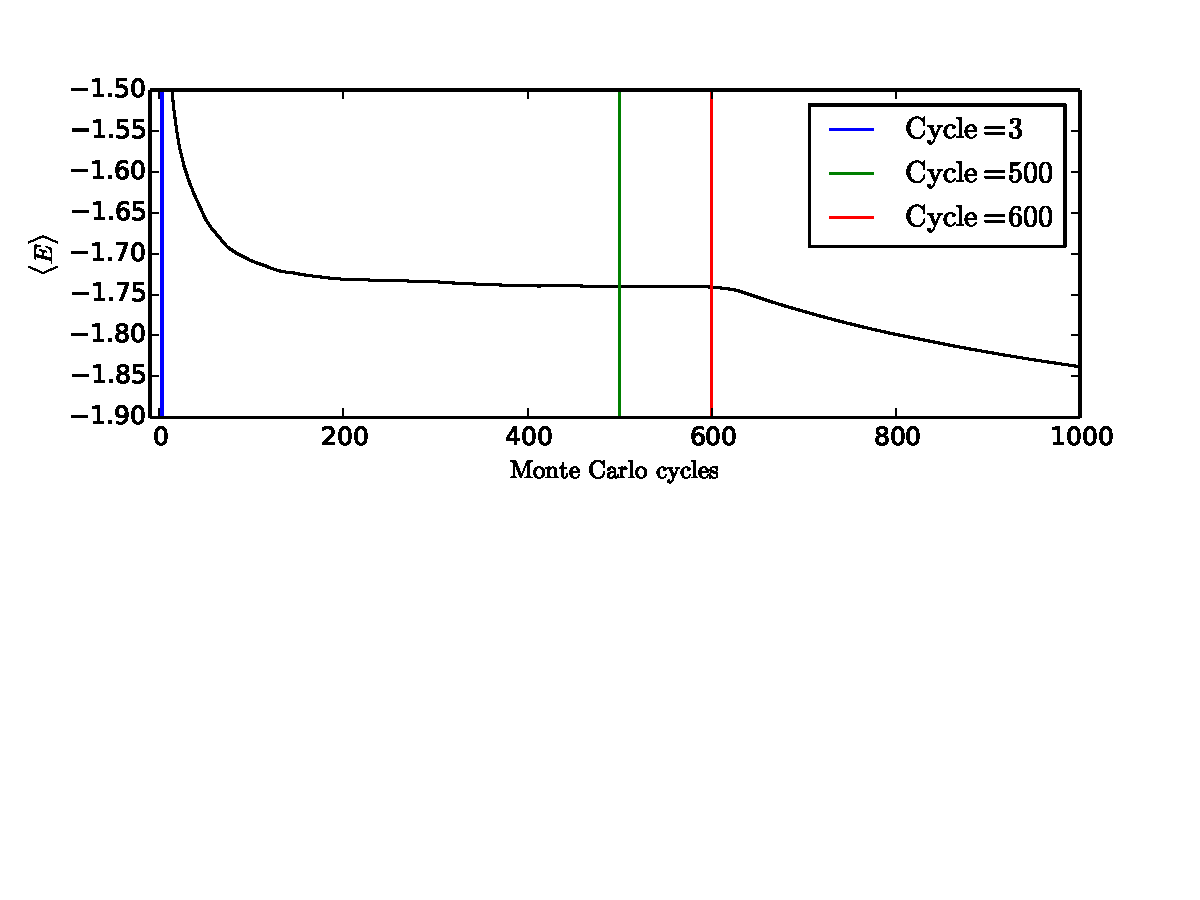
\includegraphics[scale=0.7, clip=true, trim=0 200 0 0]{../Results/extra/extra_marked.pdf}
			    \end{subfigure}
			    \caption{Snapshots of the animation. The starting position is random, reflected in the figure for cycle=3. As time goes, we get a division of the lattice in two parts as in the figure for cycle=500. Cycle=600 is around the point at which the division falls apart. The system then goes toward it's minimal energy state.}
			    \label{fig: animation snapshots}
			\end{figure}

\section{Conclusion}
	The Ising model provides a good numerical model on real physical systems and has here been used to calculate critical temperatures at which the phase transition happens for real solids. I have used Lars Onsagers result for the two dimensional Ising model ($kT/J=2.269$) to verify the results. I found the critical temperature to be $kT/J = 2.267$ where I used lattice sizes $L\times L$ with $L$= 20, 40, 60, 80 and 100 and the finite size scaling relation to relate the finite lattices to the infinite. 
	
	I also found a curious effect of a local minimum for the energy and animated the lattice to explain the behaviour and discussed whether the local minimum is a real physical phenomenon, or just simply a numerical curiosity. It may be a manifestation of the Weiss domain phenomenon ferromagnetic materials have, however no definite conclusion were made.

%\bibliographystyle{plain}
%\bibliography{references}


%\end{multicols}

\end{document}
